\chapter{Phương pháp phát hiện cộng đồng dựa trên mô hình BigCLAM}\label{chap:c3}
\ifpdf
    \graphicspath{{Chapter3/Chapter3Figs/PNG/}{Chapter3/Chapter3Figs/PDF/}{Chapter3/Chapter3Figs/}}
\else
    \graphicspath{{Chapter3/Chapter3Figs/EPS/}{Chapter3/Chapter3Figs/}}
\fi
Một trong những vấn đề của các thuật toán phát hiện cộng đồng hiện nay là khả năng xử lý các mạng lớn lên tới hàng triệu đỉnh và cạnh nối. Đặc biệt là bài toán phát hiện cộng đồng chồng chéo càng là một vấn đề. Năm 2012, đồng tác giả hai nhà khoa học Yang and Leskovec
[2012] \cite{yang2012community} đã đề giới thiệu mô hình AGM (Community-Affiliation Graph Model) cho phướng pháp phát hiện cộng đồng chồng chéo. Và một năm sau đó họ đã đề xuất phương pháp phát hiện cộng đồng lớn dựa trên mô hình AGM và đặt tên là mô hình BigCLAM (Community Affiliation Model for BigNetworks).

Trong chương này, tôi sẽ trình bày chi tiết phương pháp phát hiện cộng đồng có tính chồng chéo dựa trên mô hình BigCLAM được đề suất bởi Yang and Leskovec [2013] \cite{yang2013overlapping}. 

\section{Mô hình BigCLAM}

Trong phần này, tôi sẽ trình bày ngắn gọn mô hình cộng đồng cho đồ thị/ mạng mà BigCLAM sử dụng. Mô hình BigCLAM phần lớn vẫn dựa trên mô hình hai nhà khoa học đề xuất là AGM, một đồ thị hai phần thể hiện sự liên kết giữa các cộng đồng và các đỉnh trong mạng (hình \ref{fig:bigclam-diagram}), được ký hiệu là $B(\mathcal{V},\mathcal{C},\mathcal{M})$. Mặc dù không giống như AGM, BigCLAM không có xác suất kết nối trên mỗi cộng đồng, nhưng thay vào đó từ mỗi cộng đồng sẽ có một trọng số liên kết đến từng phần tử. Mô hình gán một trọng số không âm $F_{vc}(v \in \mathcal{V}, c \in \mathcal{C})$ trên mỗi cạnh của đồ thị phân đôi được thể hiện như là độ liên kết của quan hệ giữa một đỉnh trong mạng đến cộng đồng.
\nomenclature[KH]{$F$}{Matrix trọng số kết nối cộng đồng}
\nomenclature[KH]{$F_u$}{Vector trọng số kết nối cộng đồng}
\nomenclature[KH]{$p(u,v)$}{Xác suất tạo ra cạnh $(u,v) \in \mathcal{E}$}
\begin{definition}(Matrix và vector trọng số kết nối cộng đồng)
	
	Một matrix không âm $F =  (F_{vc})\in \mathbb{R}^{|\mathcal{V}|\times|\mathcal{C}|}$ ($F_{vc} \geq 0$) biểu diễn các trọng số liên kết giữa các đỉnh đến các cộng đồng. Một vector không âm $F_u =  (F_{uc} \geq 0)\in \mathbb{R}^{|\mathcal{V}|}$ biểu diễn các trọng số kết nối giữa đỉnh $u$ đến tất cả các cộng đồng (Hình \ref{fig:bigclam-diagram}). Với $F$, mô hình BigCLAM sinh đồ thị $G(\mathcal{V}, \mathcal{E})$ bằng tạo các cạnh $(u,v)$ với xác suất $p\left(u,v\right)$:
	\begin{equation}\label{eq:p_uv}
		p\left(u,v\right) = 1 -\exp(-F_u\cdot F_v^T) = 1 - \exp\left(-\sum_{c\in \mathcal{C}}{F_{uc}F_{vc}}\right)
	\end{equation}
\end{definition}
\begin{figure}[H]
	\centering
	\begin{minipage}[t]{0.48\textwidth}
		\centering
		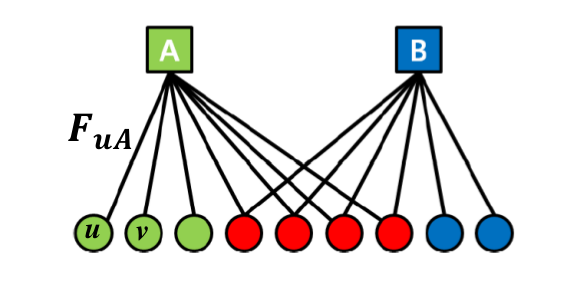
\includegraphics[width=\linewidth]{Chapter3/Chapter3Figs/bigclam-diagram}
		\caption{Mô hình cộng đồng BigCLAM}
		\label{fig:bigclam-diagram}
	\end{minipage}
	\begin{minipage}[t]{0.48\textwidth}
		\centering
		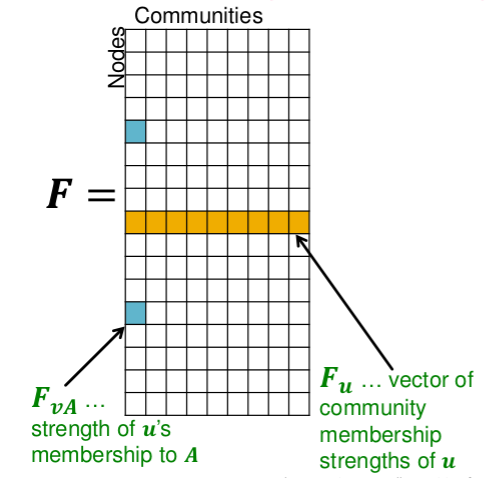
\includegraphics[width=0.7\linewidth]{Chapter3/Chapter3Figs/fmatrixvector.png}
		\caption{Matrix trọng số kết nối cộng đồng}
		\label{fig:matrixbigclam-diagram}
	\end{minipage}    
\end{figure}
Hay nói cách khác, công thức \ref{eq:p_uv} được hiểu như sau. Ta giả sử rằng mỗi cộng đồng $c \in \mathcal{C}$ kết nối đến các thành viên của nó $u,v \in \mathcal{V}$ hoàn toàn độc lập với xác suất là $1-\exp(-F_{uc}\cdot F_{vc})$ thì xác suất tạo ra cạnh $(u,v) \in \mathcal{E}$ sẽ là $1-\exp(-F_{uc}\cdot F_{vc})$. Định nghĩa này dựa trên quan sát của tác giả cho rằng với mỗi tập đỉnh là thành phần chung của sự chồng chéo các cộng đồng sẽ thu được xác suất cao hơn các tập không chồng chéo.

Công thức \ref{eq:p_uv} rõ ràng cho thấy BigCLAM tạo nên sự chồng chéo của các cộng đồng. Nó tạo ra một mối quan hệ giữa xác suất cạnh và số lượng cộng đồng chia sẻ. Điều này là do thực tế là các đỉnh chia sẻ nhiều thành viên cộng đồng nên nhận được nhiều cơ hội để tạo một cạnh trong đồ thị. Ví dụ, các cặp nút màu đỏ trong vùng chồng chéo của các cộng đồng $A$ và $B$ trong hình \ref{fig:bigclam-diagram} có hai cơ hội để tạo ra một cạnh. Đầu tiên chúng tạo ra một cạnh với xác suất $1-\exp(-F_{uA}. F_{vA})$ (do là thành viên của cộng đồng $A$) và cũng tạo ra một cạnh với xác suất $1-\exp(-F_{uB}. F_{vB})$ (do là thành viên của cộng đồng B). Như vậy xác suất cạnh giữa các đỉnh này là $1-\exp(-F_{uA}. F_{vA}  + F_{uB}. F_{vB})$. 

\section {Phát hiện cộng đồng sử dụng mô hình BigCLAM}
Với đồ thị $G(\mathcal{V},\mathcal{E})$ cho trước, mục tiêu là phát hiện ra $\mathcal{K}$ cộng đồng bằng cách tìm matrix $\hat{F} \in \mathbb{R}^{\mathcal{V}\times \mathcal{K}}$. Trong mục \ref{df:dn-likelihood} sẽ trình bày phương pháp xác định $\hat{F}$ thông qua việc tìm cực đại hàm khả dĩ (định nghĩa \ref{df:MLE}) $l(F) = \log P(G,F)$ 

\subsection {Cực đại hàm khả dĩ ma trận trọng số liên kết của đồ thị}\label{df:dn-likelihood}
	
	Cho $G(\mathcal{V},\mathcal{E})$ là một đồ thị với tập cạnh $\mathcal{E}$ và tập đỉnh $\mathcal{V}$, với $F=(F_{vc})\in \mathbb{R}^{|\mathcal{V}|\times|\mathcal{K}|} (v \in \mathcal{V}, c \in \mathcal{C})$ là một matrix trọng số liên kết (ở đây $\mathcal{K}$ là số cộng đồng).
	
Với mô hình trên, ta có thể thấy rằng xác suất để một tạo một cạnh $(u,v)$ trong đồ thị là $p(u,v)$ và ngược lại là $1-p(u,v)$ hay có thể viết lại như sau:
\begin{eqnarray}
	p((u,v) \in \mathcal{E}|F) = p(u,v)\\
	p((u,v) \notin \mathcal{E}|F) = 1-p(u,v)
\end{eqnarray}

Xét toàn bộ đồ thị $G(\mathcal{V},\mathcal{E})$ ta có được $P(G|F)$ chính là khả dĩ của $F$ sinh ra đồ thị $G$ như sau:
\begin{equation}
\begin{array}{lll}
	\mathcal{L}(F|G) = P(G|F)
	&= \prod_{(u,v) \in \mathcal{E}}{p(u,v)}\prod_{(u,v) \neq \mathcal{E}}{(1-p(u,v))}\\
	&= \prod_{(u,v) \in E}{(1 - \exp(-F_uF_v^T))}\prod_{(u,v) \neq \mathcal{E}}{\exp(-F_uF_v^T)}.
\end{array}
\end{equation}
Đây là một dang bài toán ước lượng tham số bằng cực đại hàm khả dĩ (Maximum likelihood estimation). Theo định nghĩa \ref{df:MLE} ta được hàm log-likelihood $l(F)$ sau:
\begin{equation}\label{ct:loglikelihood}
	l(F) = log \mathcal{L}(F|G) = \sum_{(u,v) \in \mathcal{E}}{(log(1-\exp(-F_uF_v^T)) - \sum_{(u,v)\neq \mathcal{E}}{\exp(F_uF_v^T})}.
\end{equation}
Mặt khác hàm logarit là đơn điệu tăng nên $\hat{F}$ cực đại $l(F)$ thì cũng là cực đại log $P(G|F)$ tức là:

\begin{equation} \label{eq:ctf_hat}
	\hat{F} = \arg \max_{F \geq 0} \mathcal{L}(F) = \arg \max_{F \geq 0} l(F) 
\end{equation}

Từ công thức \ref{ct:loglikelihood}, ta giả sử với $\mathcal{K}$ cộng đồng đã biết (phương pháp tìm $\mathcal{K}$ sẽ được đề cập ở phần sau) ta cần giải quyết bài toán trong công thức \ref{eq:ctf_hat}. Nhưng thay vì phải cực đại $l(F)$ ta sẽ tách thành các bài toán tìm cực đại $l(F_u)$ và cập nhật lại $F_u$ trên từng đỉnh $u \in \mathcal{V}$ theo các $F_v,v\neq u$ như sau:

\begin{equation}\label{eq:ctfu_hat}
\hat{F_u} = \arg \max_{F_{uc}, c \in \mathcal{C}} l(F_u) 
\end{equation}
Trong đó: 
\begin{equation}\label{eq:ctfu_l}
l(F_u) = \sum_{v \in \mathcal{N}(u)}{log(1 - \exp(-F_u F_v^T))} - \sum_{v \notin \mathcal{N}(u)}{F_uF_v^T}
\end{equation}
$\mathcal{N}(u)$ là tập các đỉnh lân cận của $u$ (Định nghĩa \ref{df:dinhlancan})

Ta thấy rằng $l(F_u)$ là một hàm lõm như vậy vấn đề trên được coi như là bài toán tối ưu hàm lõm và có thể tìm được điểm cực đại duy nhất một cách dễ dàng. Để ước lượng được các vector $F_u$ (công thức \ref{eq:ctfu_hat}) ta sử dụng các phương pháp tối ưu hàm lồi/ lõm được trình bày ở mục \ref{muc:toiuuhamloi}
\begin{equation}\label{eq:gradian}
l'(F_u) = l(F_u)+\alpha \bigtriangledown(l(F_u))
\end{equation}
Trong đó građian cho log-likelihood của $F_u$ là:
\begin{equation}\label{eq:ctfu_l1}
\bigtriangledown(l(F_u))=\dfrac{\partial l(F_u)}{\partial F_u} = \sum_{v \in \mathcal{N}(u)}{F_v \dfrac{\exp(-F_u F_v^T)}{1-\exp(-F_u F_v^T)}} - \sum_{v \notin \mathcal{N}(u)}{F_v}
\end{equation}

Để giảm độ phức tạp tính toán xuống còn $O(|\mathcal{N}(u)|)$ tôi xin biến đổi lần lượt các công thức \ref{eq:ctfu_l} \ref{eq:ctfu_l1} như sau:

\begin{equation}\label{eq:caitien}
\sum_{v \notin \mathcal{N}(u)} {F_u F_v^T}= \sum_{v} {F_u F_v^T} - \sum_{v \in N(u)} {F_u F_v^T}
\end{equation}

\begin{equation}\label{eq:caitien1}
\sum_{v \notin \mathcal{N}(u)} {F_v}= \left(\sum_{v} {F_v}\right) - F_u - \left(\sum_{v \in \mathcal{N}(u)} {F_v}\right)
\end{equation}

Matrix $F$ được cập nhật sau mỗi vòng lặp theo công thức \ref{eq:gradian}. Ta nên cho thuật toán hội tụ khi:
 \begin{equation}
 \dfrac{l'{(F_u)} - l(F_u)}{l(F_u)} < 0.0001, \forall u \in \mathcal{V}
 \end{equation}

\subsection{Khởi tạo tạo ma trận trọng số liên kết cộng đồng}
Kết quả của bài toán phát hiện cộng đồng ảnh hưởng rất nhiều từ việc khởi tạo giá tri $F_u, u\in \mathcal{V}$ cho quá trình tối ưu hàm lồi/ lõm. Để khởi tạo matrix $F$ (Định nghĩa \ref{dn:initF}), ta chọn sử dụng phương pháp tìm vùng lân cận địa phương nhỏ nhất của Gleich and Seshadhri [2011] \cite{DBLP:journals/corr/abs-1112-0031} đã được đề cập đến trong định nghĩa \ref{df:dodan} và định nghĩa \ref{df:dinhlancan}

\begin{definition}(Khởi tạo matrix trọng số liên kết)\label{dn:initF}
	
	Gọi $F$ là một matrix trọng số liên kết. $F$ được khởi tạo như sau:
	\begin{equation}
		F_{(u^{\prime})(N(u))} =
			\begin{cases}
			1 & \textit{Nếu $u^{\prime} \in N(u)$ và $N(u)$ là vùng lân cận địa phương nhỏ nhất của $u$} \\
			0 & \textit{Trường hợp còn lại}
			\end{cases}
	\end{equation}
\end{definition}
\subsection{Xác định các liên kết cộng đồng}

Sau khi công thức \ref{eq:ctf_hat} hội tụ, ta sẽ có được một matrix trọng số liên kết $F$. Tuy nhiên ta cần phải xác định đỉnh $u$ có thuộc cộng đồng $c$ hay không. Vì vậy ta phải lựa chọn một ngưỡng $\delta$ cho matrix $F$ qua định nghĩa \ref{dn:xacdinhlienketcd}.
\begin{definition}(Xác định liên kết cộng đồng) \label{dn:xacdinhlienketcd}
	Cho $G(\mathcal{V},\mathcal{E})$, $F$ là matrix trọng số liên kết của $G$ và $\epsilon = \dfrac{2|E|}{|V|(|V| - 1)}$.
	
	Thuật toán xét $u \in \mathcal{V}$ như một thành viên trong cộng đồng $c\in \mathcal{C}$ nếu thỏa mãn $F_{uc}\geq \delta = \sqrt{-\log(1-\epsilon)}$.
\end{definition}

\subsection{Xác định số cộng đồng}
Trong phần đầu của chương này đã tiền hành xây dựng mô hình với giả sử $\mathcal{K}$ số cộng đồng trong $G(\mathcal{V},\mathcal{E})$ đã biết. Yang và Leskovec đã trình bày một phương pháp để ước lượng gần nhất số cộng đồng $\mathcal{K}$ vẫn dựa trên phương pháp cực đại hàm khả dĩ như sau:
\begin{itemize}
	\item Chọn ngẫu nhiên $20\%$ cặp đỉnh cho $H$;
	\item Với mỗi $\mathcal{K}$ là số cộng đồng. $\mathcal{K} \in [minCom;maxCom]$ với bước nhảy trong khoảng $[minCom; maxCom]$ là $\alpha = \exp{\left(\log{\left(\dfrac{maxCom}{minCom}\right)}\times\dfrac{1}{divCom}\right)}$. Trong đó $minCom$ là số cộng đồng nhỏ nhất, $maxCom$ là số cộng đồng lớn nhất và $divCom$ là số lượng $\mathcal{K}$ muốn thử.
	\begin{itemize}
			\item Chạy thuật toán phát hiện cộng đồng, với $\mathcal{K}$ là số cộng đồng mong muốn pháy hiện
			\item Đánh giá likelihood của matrix trọng số trên tập $H$, $l_k{(F_H)}$.
		\end{itemize}
	\item $\hat{\mathcal{K}} = \arg \max_K l_k{(F_H)}$.
\end{itemize} 

\section{Đánh giá hiệu năng}
Theo kết quả của các tác giả khi so sánh hiệu năng  giữa giữa BigCLAM và các mô hình được sử dụng để phát hiện cộng đồng như LC \cite{ahn2010link}, CPM \cite{palla2005uncovering}, MMS \cite{airoldi2008mixed}. Hình \ref{fig:bigclamcomparis} cho thấy BigCLAM cho hiệu năng cao hơn từ $10$ đến $100$ lần so với phương pháp còn lại. 

\begin{figure}[H]
	\centering
	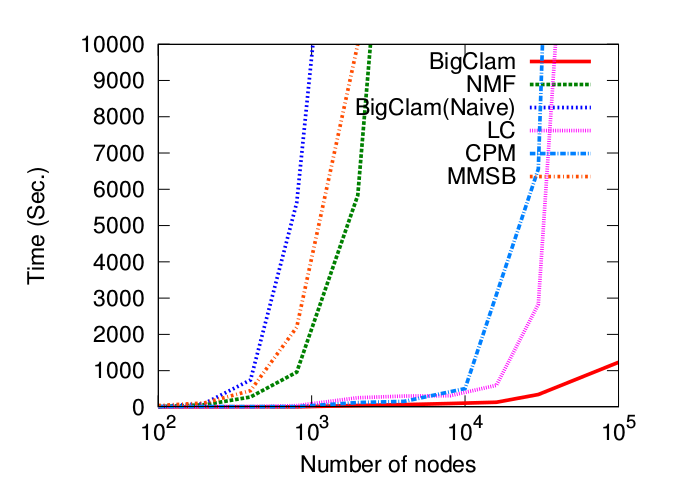
\includegraphics[width=0.6\linewidth]{Chapter3/Chapter3Figs/bigclamcomparis}
	\caption{So sánh hiệu năng của các mô hình với BigCLAM}
	\label{fig:bigclamcomparis}
\end{figure}

Ngoài ra các tác giả sử dụng một số mạng đã được xác định trước các cộng đồng (ground-truth communities) để đánh giá độ chính xác của các mô hình được dùng để phát hiện cộng đồng. Bảng \ref{comtruth} dưới đây là thông tin các mạng được sử dụng.

\begin{table}[H]
	\centering
	\caption{Mô tả các mạng sử dụng để thực nghiệm}
	\label{comtruth}
	\begin{tabular}{@{}lrrr@{}}
		\toprule
		Tên mạng                & Số đỉnh      & Số cạnh         & Số cộng đồng \\ \midrule
		Mạng xã hội LiveJournal & $3,997,962$  & $34,681,189$    & $287,512$    \\
		Mạng xã hội Friendster  & $65,608,366$ & $1,806,067,135$ & $957,154$    \\
		Mạng xã hội Ourkut      & $3,072,441$  & $117,185,083$   & $6,288,363$  \\
		Mạng xã hội Youtube     & $1,134,890$  & $2,987,624$     & $8,385$      \\
		Mạng cộng tác DBLP      & $317,080$    & $1,049,866$     & $13,477$     \\
		Mạng bán hàng Amazon    & $334,863$    & $925,872$       & $75,149$     \\ \bottomrule
	\end{tabular}
\end{table}
Tác giả sử dụng các thang đo đánh giá như sau:
\begin{itemize}
	\item \textbf{Average $F1$ score} \citep{1742-5468-2011-02-P02017} : Thể hiện mức độ chính xác trung bình của các cộng đồng phát hiện được với các cộng đồng thực tế.
	\item \textbf{Omega Index} \cite{gregory2011fuzzy}: Là chỉ số thể hiện độ chính xác số cộng đồng mà mỗi đỉnh thuộc.
	\item \textbf{Accuracy in the number of communities}:Độ chính xác về số lượng cộng đồng
\end{itemize}
Hình \ref{fig:ground-truthcommunities} là kết quả của sự so sánh hiệu năng giữa các mô hình trên một số mạng. Dễ dàng thấy được, hiệu năng trung bình của mô hình BigCLAM là $3.60$ cao hơn hơn các mô hình còn lại như Link Clustering ($2.01$), CPM ($2.47$) và MMSB ($3.14$). Nhìn chung, BigCLAM có hiệu năng tương đối tốt, tỏ ra khá vượt trội so với các phương pháp thường được sử dụng và nó có khả năng phát hiện đa dạng các loại cộng đồng (chồng chéo, không chồng chéo, lồng nhau).
\begin{figure}[H]
	\centering
	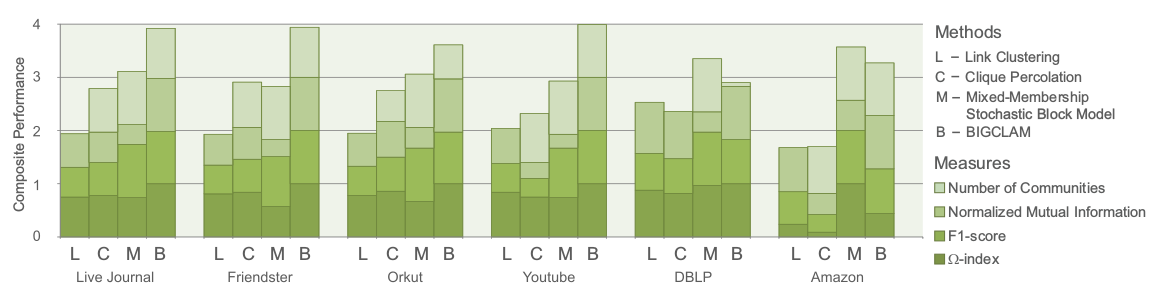
\includegraphics[width=\linewidth]{Chapter3/Chapter3Figs/ground-truthcommunities.png}
	\caption{Biểu đồ so sánh độ chính xác các mô hình trên các mạng biết trước cộng đồng}
	\label{fig:ground-truthcommunities}
\end{figure}

Mô hình BigCLAM dựa trên kỹ thuật NMF, vậy nên hoàn toàn có thể tăng tốc độ trên các kỹ thuật xử lý song song và phân tán. Trong chương \ref{chap:c4} giới thiệu và đề xuất phương pháp tăng tốc bài toán dựa trên sức mạnh xử lý trên cụm máy tính.
